\documentclass[11pt,a4paper]{article}

\usepackage[left=2cm,text={17cm,24cm},top=3cm]{geometry}
\usepackage[english]{babel}
\usepackage[utf8]{inputenc}
\usepackage[T1]{fontenc}

\usepackage{url}
\usepackage{tikz}
\usepackage{float}
\usepackage{xcolor}
\usepackage{siunitx}
\usepackage{amsmath}
\usepackage{accents}
\usepackage{comment}
\usepackage{listings}
\usepackage{csquotes}
\usepackage{hyperref}
\usepackage{textcomp}
\usepackage{amsfonts}
\usepackage{breakurl}
\usepackage{etoolbox}
\usepackage{graphicx}
\usepackage{multicol}
\usepackage{multirow}
\usepackage{indentfirst}
\usepackage{supertabular}
\usepackage[titles]{tocloft}

\def\UrlBreaks{\do\/\do-} % URL breaking characters

\definecolor{urlcolor}{RGB}{6, 69, 173}

\newcommand{\red}[1]{\textcolor{red}{#1}} % \red{text in red}
\newcommand{\blue}[1]{\textcolor{blue}{#1}} % \blue{text in blue}
\newcommand{\TODO}{\textbf{\textcolor{red}{TODO}}} % red bold TODO
\newcommand{\tilda}{\raisebox{0.5ex}{\texttildelow}} % command \tilda for '~' character

\renewcommand{\cftdot}{}

\setlength\parindent{0pt} % do NOT indent
\graphicspath{{../}} % path to images

\patchcmd{\thebibliography}{\section*{\refname}}{}{}{}

\begin{document}

\begin{titlepage}

    \begin{center}
        % FIX: lines must end with '%', if not then it will result in an incorrect centering
        \vfill {%
            \Huge{%
                \textsc{%
                    Faculty of Informatics\\[3mm]%
                    Masaryk University%
                }%
            }%
        }%

        \hfill\\[15mm]

        \begin{figure}[!h]
            \centering
            
\includegraphics[scale=3]{doc/img/muni-fi-logo.pdf}
        \end{figure}

        \hfill\\[10mm]

        \Huge{
            \textbf{
                PA181
            }
        }

        \hfill\\[-10mm]

        \huge{
            \textbf{
                Services - Systems, Modeling and Execution
            }
        }

        \hfill\\[10mm]

        \LARGE{
            \textbf{
                Term Project Documentation
            }
        }
        \vfill

    \end{center}

        \Large{
            \hfill\\
            Adrián Tóth (491322)\\
            Jiří Čechák (445717)\\
            Jan Ondruch (433341)\\
            Tadeáš Pavlík (487555)\\
            Václav Stehlík (487580) \hfill \today
        }

\end{titlepage}

\setlength{\parskip}{0pt}
    \hypersetup{hidelinks}\tableofcontents
\setlength{\parskip}{0pt}

\newpage

\section{About}

Term project for course \textit{PA181 Services - Systems, Modeling and Execution}\footnote{\href{https://is.muni.cz/predmet/fi/jaro2019/PA181}{\color{urlcolor}{is.muni.cz/predmet/fi/jaro2019/PA181}}} in year 2019. Within the project, we had to create a fully functional application using the \textit{IBM Cloud}\footnote{\href{https://cloud.ibm.com/}{\color{urlcolor}{cloud.ibm.com}}} technology including a detailed documentation and a presentation. \textit{doc. Mouzhi Ge, Ph.D.}\footnote{\href{https://is.muni.cz/auth/osoba/239833}{\color{urlcolor}{is.muni.cz/auth/osoba/239833}}} is the project supervisor.

\section{Idea}

The core idea was to create and develop a useful and practical application. The application provide services for testing the users in a form of questions and answers. Users are able to test themselves via these questions by selecting the correct answers. There are severals tests in three different types of language (Czech, Slovak and English).

\section{Used Technologies}

The following technologies were integrated and used during the development process:
\begin{itemize}
    \item cloud based platform
    \begin{itemize}
        \item IBM Cloud
    \end{itemize}

    \item version control system (VCS)
    \begin{itemize}
        \item GitHub\footnote{\href{https://github.com/}{\color{urlcolor}{github.com}}}
    \end{itemize}

    \item continuous integration (CI)
    \begin{itemize}
        \item Travis CI\footnote{\href{https://travis-ci.org/}{\color{urlcolor}{travis-ci.org}}}
    \end{itemize}
\end{itemize}

Besides the used technologies we were using additional available tools such as:
\begin{itemize}
    \item IBM Cloud DevOps Toolchain
    \begin{itemize}
        \item Set or combination of tools that build and deploy the software in a repeatable way with minimal human intervention.
    \end{itemize}

    \item React
    \begin{itemize}
        \item A JavaScript library for building user interfaces.
    \end{itemize}

    \item ASP.NET
    \begin{itemize}
        \item A framework for building web apps and services with .NET and C\#.
    \end{itemize}
\end{itemize}

\section{Work Division}

Our team consisted of 5 members: Adrián Tóth, Jan Ondruch, Jiří Čechák, Tadeáš Pavlík and Václav Stehlík.\\

Everyone from us was in charge of a certain part of the project. The work was divided as the following:
\begin{itemize}
    \item Adrián Tóth
    \begin{itemize}
        \item project initialization
        \item VCS initialization
        \item creation of project skeleton
        \item Travis CI integration and configuration
        \item IBM DevOps toolchain configuration
        \item creation of continuous delivery pipeline
        \item project deployment
        \item bug fixing
        \item documentation
    \end{itemize}

    \item Jan Ondruch
    \begin{itemize}
        \item user research
        \item specifications
        \item application design (idea)
        \item testing (user interface)
        \item testing (usability)
    \end{itemize}

    \item Jiří Čechák
    \begin{itemize}
        \item application design (user interface)
        \item application user interface initialization (framework, layout, views)
        \item application frontend
        \item testing (user interface)
        \item bug fixing
    \end{itemize}

    \item Tadeáš Pavlík
    \begin{itemize}
        \item analysis
        \item application design (concept)
        \item application design (user interface)
        \item application backend \TODO
        \item testing (blackbox)
    \end{itemize}

    \item Václav Stehlík
    \begin{itemize}
        \item application design (concept)
        \item application backend
        \item backend and frontend interconnection
        \item troubleshooting
        \item bug fixing
    \end{itemize}
\end{itemize}

\section{References}

Domain names of the deployed application are:
\begin{itemize}
    \item \href{https://pa181.eu-de.mybluemix.net/}{\color{urlcolor}{pa181.eu-de.mybluemix.net}}
    \item \href{https://pa181.eu-de.cf.appdomain.cloud/}{\color{urlcolor}{pa181.eu-de.cf.appdomain.cloud}}
\end{itemize}

Source code of the application can be found at:
\begin{itemize}
    \item \href{https://github.com/europ/MUNI-FI-PA181/tree/master/src}{\color{urlcolor}{github.com/europ/MUNI-FI-PA181/tree/master/src}}
\end{itemize}

Setup guide for the application can be found at:
\begin{itemize}
    \item \href{https://github.com/europ/MUNI-FI-PA181/wiki/Setup}{\color{urlcolor}{github.com/europ/MUNI-FI-PA181/wiki/Setup}}
\end{itemize}

Documentation of the application can be found at:
\begin{itemize}
    \item \href{https://github.com/europ/MUNI-FI-PA181/blob/master/doc/doc.pdf}{\color{urlcolor}{github.com/europ/MUNI-FI-PA181/blob/master/doc/doc.pdf}}
\end{itemize}

Presentation of the application can be found at:
\begin{itemize}
    \item \href{https://github.com/europ/MUNI-FI-PA181/blob/master/pres/pres.pdf}{\color{urlcolor}{github.com/europ/MUNI-FI-PA181/blob/master/pres/pres.pdf}}
\end{itemize}

\section{Application initialization}

Firstly, we have chosen a stable, reliable and safe platform supporting team project development - GitHub. Furthermore, GitHub provides a version control system management and the integration with IBM Cloud is supported. Subsequently, after the repository was configured properly, we had to choose the technologies. We decided to use \#C (general-purpose, multi-paradigm and object oriented programming language) and React (library for building user interfaces) for the project. Based on the above, we have initialized the project skeleton - a \textit{'Hello, World!'} application.

\section{Application implementation}

The project was implemented via \textit{ASP.NET} framework using a Model--view--controller as an architectural pattern. The core UI was implemented in JavaScript using React library. This UI was later interconnected with backend. Our application supports an application log too to find easier the fatal failures. Our application was divided into few parts that communicate together and process requests - API, entities, repositories and services. The requests are firstly processed in the API, more precisely endpoint in controller. To process this request, the required actions are delegated to services (the business logic specific for our application is implemented here) that delegates the related subrequests to repository that provides the database communication using wrappers. \TODO

\section{Application deployment}

The deployment was configured before the core implementation itself. Deployment was initialized and configured on the already set \textit{'Hello, World!'} application. We wanted to create a fully automated delivery with zero intervention required, which allowed us to concentrate and focus on code only instead of problematic deployment. We were using a continuous delivery approach - automated build and deploy method via IBM's delivery pipeline. The delivery pipeline was configured to automatically install all required dependencies, build and deploy the application. The development process required to just commit the changes into the version control repository.\\

Whole deployment is based on one own properly configured DevOps toolchain. The toolchain is shown in Figure \ref{fig:toolchain}, which includes GitHub\footnote{\href{https://console.bluemix.net/docs/services/ContinuousDelivery/toolchains\_integrations.html\#github}{\color{urlcolor}{console.bluemix.net/docs/services/ContinuousDelivery/toolchains\_integrations.html\#github}}}, Travis CI\footnote{\href{https://console.bluemix.net/docs/services/ContinuousDelivery/toolchains\_integrations.html\#othertool}{\color{urlcolor}{console.bluemix.net/docs/services/ContinuousDelivery/toolchains\_integrations.html\#othertool}}} (as other tool) and Delivery Pipeline\footnote{\href{https://console.bluemix.net/docs/services/ContinuousDelivery/toolchains\_integrations.html\#deliverypipeline}{\color{urlcolor}{console.bluemix.net/docs/services/ContinuousDelivery/toolchains\_integrations.html\#deliverypipeline}}}.

\begin{figure}[H]
    \centering
    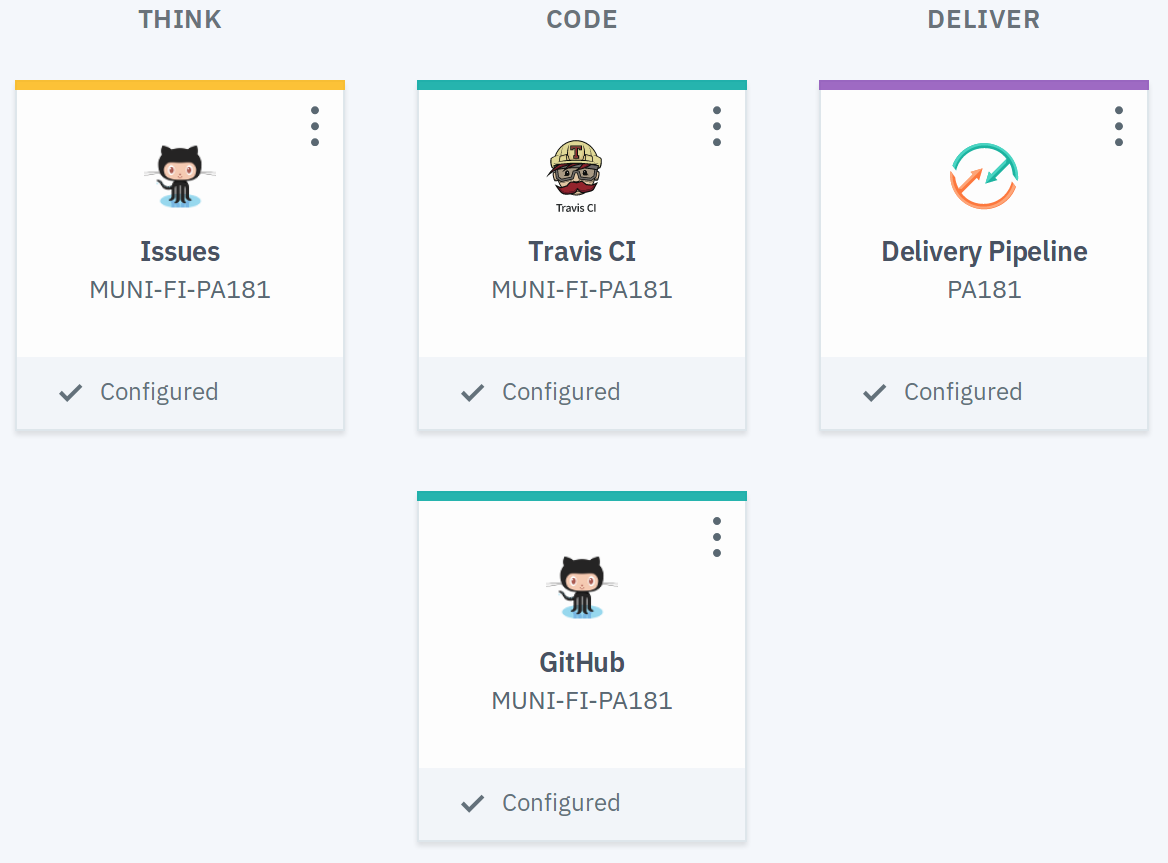
\includegraphics[scale=0.3]{img/toolchain.png}
    \caption{Toolchain}
    \label{fig:toolchain}
\end{figure}

The toolchain providing a continuous delivery service allows us to focus on code only. After the continuous delivery toolchain was set properly, we just had to commit the changes to the repository and the application was immediately built and deployed.

\section{Application instructions}

\TODO: how to use, tutorial, examples

\section{Screenshots}

\TODO: images (add it to 'doc/img' folder - vector would be the best or raster with high resolution)

\section{Development issues}

During the project development we have faced a few problems that have been reported:
\begin{itemize}
    \item \href{https://github.com/IBM-Bluemix-Docs/ContinuousDelivery/issues/13}{\color{urlcolor}{\color{urlcolor}}{github.com/IBM-Bluemix-Docs/ContinuousDelivery/issues/13}}
    \item \href{https://github.com/IBM-Cloud/aspnet-core-helloworld/issues/39}{\color{urlcolor}{github.com/IBM-Cloud/aspnet-core-helloworld/issues/39}}
\end{itemize}

\end{document}
